\documentclass[conference]{IEEEtran}

\usepackage[T1]{fontenc}

\usepackage{graphicx}

\usepackage{url}

\begin{document}

\title{Predictive Maintenance via Sensor Features and Sequence Models}

\author{\IEEEauthorblockN{MS Thejas, Deepak Pandey, Tathagat Harsh, Aryan, Garv Verma}\IEEEauthorblockA{CSAI Project 7 -- Phase Two}}

\maketitle

\begin{abstract}

We estimate remaining useful life (RUL) on NASA C-MAPSS FD001 using engineered-feature Random Forest regression, a 30-cycle LSTM, and a joint feature-sequence hybrid. All models use the same 80 training engines, 20 validation engines and 100 official test engines. We retain the Phase One 125-cycle target cap and report both capped and uncapped errors. Three random initializations quantify neural training variability. Validation selects RandomForest. The paired interval includes zero; a reliable hybrid advantage is not established. This is an academic benchmark, not an operational maintenance policy.

\end{abstract}

\section{Motivation and literature}

Phase One uses fixed rolling statistics. Such summaries can discard temporal order and interactions, motivating a sequence encoder. NASA's run-to-failure simulator supplies multivariate trajectories with known terminal labels [1]. Hochreiter and Schmidhuber introduced gated memory cells to support learning across time [2]. Our LSTM uses this gating mechanism within a finite window; it does not claim whole-lifetime memory. Bai, Kolter and Koltun show temporal convolutions are a credible alternative across sequence tasks [3]; their general benchmark does not establish superiority on FD001. A temporal CNN is a future comparison, not an implemented result.

\section{Dataset, target and split}

FD001 contains 100 run-to-failure training engines and 100 truncated test engines, with 21 sensors and 3 settings. Training RUL is max cycle within engine minus current cycle. Only training trajectories use that formula; official test endpoint labels come from RUL\_FD001.txt. Targets are min(RUL,125), explicitly inherited from Phase One.

Engine IDs are shuffled using NumPy seed 2026, with 80/20 train/validation allocation persisted in the manifest. Official test IDs inhabit a separate dataset namespace. One pseudo-truncated endpoint per validation engine is selected with a fixed RNG independently of model predictions. All training cycles are used. The final benchmark intentionally retains the 80-engine fitted models so that every model has exactly the same training information; it is not directly comparable to the Phase One model trained on all 100 engines.

The loader rejects missing/nonfinite values, invalid IDs, duplicate cycles and gaps. Flat sensors are detected only on the 80 training engines (standard deviation $\leq$1e-8). StandardScaler is fitted only there. FD001 has one operating regime, so per-regime normalization reduces to global training-only normalization and a constant regime feature is omitted. Sensor inspection is exported. The single-regime assumption must not be extended blindly to FD002/FD004.

\section{Features and architecture}

The regression baseline receives cycle age, current sensor readings, trailing means, standard deviations and least-squares slopes over 5 and 10 cycles, and each sensor's deviation from its first observation. All features are causal and reset at engine boundaries. Initial-value deviations can be sensitive to a noisy first measurement.

The LSTM input is a 30 x S normalized sensor matrix. Histories shorter than 30 repeat the first available row on the left. A single 32-unit LSTM supplies its final hidden state to Linear(32,32), ReLU, Dropout(0.2), Linear(32,1), Sigmoid; predictions are multiplied by 125. The hybrid adds a Linear(F,16), ReLU branch on standardized engineered features, concatenated with the LSTM state before the same regression head (input width 48). This is joint feature fusion rather than an arbitrary average of model predictions. It tests whether explicit age and degradation summaries complement learned sequence features.

For LSTM gates i, f, o and candidate g, cell state c\_t=f\_t*c\_(t-1)+i\_t*g\_t and hidden state h\_t=o\_t*tanh(c\_t). Sigmoid gates determine information retention. The loss is mean squared error on y/125. The bounded output supports the capped task but cannot represent RUL above 125; uncapped early-life error therefore has a structural floor.

\section{Optimization and regularization}

AdamW uses learning rate 0.001 and weight decay 0.0001, batch size 256 and gradient norm clipping at 1. Maximum epochs: 60; patience: 10. The best validation RMSE checkpoint is restored. Seeds [42, 43, 44] are used for each DL configuration, with deterministic CPU operations and 4 Torch threads. Architecture selection uses mean validation RMSE across seeds, not official test results. The Random Forest uses 200 trees, leaf size 3, max-features 0.8 and seed 42. It is a fresh fair-split AML comparator rather than reuse of the Phase One all-engine checkpoint.

\section{Ablation and evaluation protocol}

LSTM1 removes temporal context while retaining the recurrent architecture. LSTM30\_no\_dropout changes only head dropout to zero. Hybrid30 adds the engineered branch to LSTM30; parameter count also changes, so this is not a parameter-matched proof that features alone cause a difference. Other regularizers remain enabled in the no-dropout ablation. Each model predicts exactly the last observed cycle of each official test engine.

RMSE=sqrt(mean((prediction-truth)\textasciicircum{}2)); MAE=mean(abs(prediction-truth)). NASA score sums exp(-error/13)-1 for negative errors and exp(error/10)-1 otherwise. Positive error overestimates remaining life. Stage bands use uncapped truth: late 0-30, middle 31-90, early $>$90 cycles. These are analysis definitions, not certified maintenance thresholds.

\section{Results}

Mean test metrics across seeds (cycles; Random Forest has one run):

\begin{table}[ht]

\centering\caption{Mean test errors in cycles. C: capped; U: uncapped.}

\begin{tabular}{lcrr}\hline Model & Target & RMSE & MAE\\\hline

Hybrid30 & C & 14.510 & 10.427 \\

Hybrid30 & U & 15.517 & 11.497 \\

LSTM1 & C & 16.747 & 11.522 \\

LSTM1 & U & 17.721 & 12.592 \\

LSTM30 & C & 14.585 & 10.760 \\

LSTM30 & U & 15.678 & 11.830 \\

LSTM30\_no\_dropout & C & 14.147 & 10.329 \\

LSTM30\_no\_dropout & U & 15.343 & 11.399 \\

RandomForest & C & 12.953 & 9.318 \\

RandomForest & U & 14.156 & 10.388 \\

\hline\end{tabular}\end{table}

Per-seed metrics and standard deviations are in reports/test\_metrics.csv and reports/summary.csv. Learning curves record both training and validation RMSE; plots show the first seed for clarity. Engine-level predictions and stage metrics are exported, not inferred from plots.

For seed-averaged predictions, a paired 2,000-resample engine bootstrap estimates the Hybrid30-minus-LSTM30 capped RMSE difference with a 95\% percentile interval [-2.536, 1.997] cycles. Negative means the hybrid is better. The paired interval includes zero; a reliable hybrid advantage is not established. This ensemble comparison differs from mean per-seed RMSE and is labeled accordingly. The interval conditions on the fitted training split; it does not include split-selection uncertainty.

Against LSTM30, the one-cycle ablation changes mean capped test RMSE by +2.162 cycles; removing dropout changes it by -0.438 cycles. Positive differences are worse. These are descriptive results from the pre-specified comparisons, not a reason to retune against the test set.

Uncapped stage errors (mean across seeds):

RandomForest: late\_0\_30: RMSE 5.88, MAE 4.28; middle\_31\_90: RMSE 14.94, MAE 10.81; early\_over\_90: RMSE 16.62, MAE 13.44 cycles.

LSTM30: late\_0\_30: RMSE 6.89, MAE 5.61; middle\_31\_90: RMSE 20.30, MAE 15.57; early\_over\_90: RMSE 15.70, MAE 12.86 cycles.

Hybrid30: late\_0\_30: RMSE 5.03, MAE 4.00; middle\_31\_90: RMSE 16.46, MAE 12.38; early\_over\_90: RMSE 18.38, MAE 15.02 cycles.

\section{Limitations and conclusions}

Sequence modeling addresses the information discarded by rolling summaries, but predictive gains must be read from the measured comparison. The optional hybrid requirement is satisfied by implementing and testing a technically motivated combination; additional marks are at the evaluator's discretion, and a gain is not assumed. Only one engine split and a small validation set are used. Overlapping training windows are correlated and long-lived engines contribute more samples. Three seeds quantify initialization variability only. No broad hyperparameter search, external dataset validation, uncertainty calibration or real-engine trial is claimed. The test set must not be reused for subsequent tuning. FD001's simulated single-condition setting restricts generalization.

\section{Reproducibility and contribution record}

Run python -m phase2.pipeline, then python -m phase2.build\_submission. The manifest stores engine IDs, endpoints, target cap, file SHA256 values, runtime versions and seeds. Saved models and preprocessing enable label-free inference via phase2.predict. Unit tests cover causal features, within-engine padding, targets, malformed inputs, gradients and checkpoint reloads. The notebook exposes the experiment, tables and figures. Proposed member responsibilities and viva explanations are in VIVA.md; actual Phase Two contributions must be confirmed by the team and should not be fabricated.

\section{References}

[1] A. Saxena and K. Goebel, Turbofan Engine Degradation Simulation Data Set, NASA Ames Prognostics Data Repository, 2008. \url{https://www.nasa.gov/intelligent-systems-division/discovery-and-systems-health/pcoe/pcoe-data-set-repository/}

[2] S. Hochreiter and J. Schmidhuber, Long Short-Term Memory, Neural Computation, 9(8), 1735-1780, 1997. \url{https://doi.org/10.1162/neco.1997.9.8.1735}

[3] S. Bai, J. Z. Kolter and V. Koltun, An Empirical Evaluation of Generic Convolutional and Recurrent Networks for Sequence Modeling, 2018. \url{https://arxiv.org/abs/1803.01271}

\begin{figure}[ht]\centering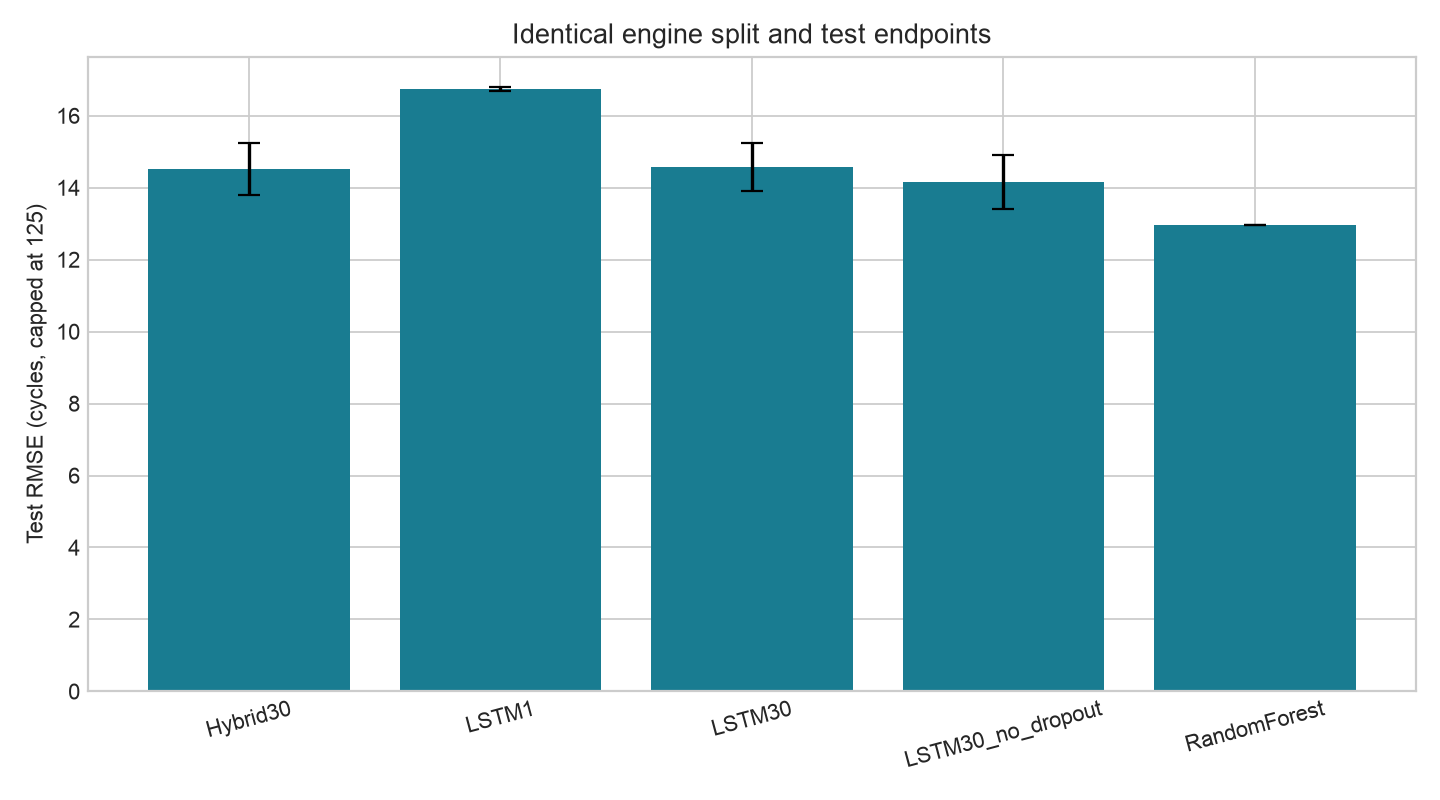
\includegraphics[width=\columnwidth]{../reports/comparison.png}\caption{Capped test RMSE; error bars show standard deviation across initializations, not a confidence interval.}\end{figure}

\end{document}